\documentclass{article}
\usepackage{graphicx}
\usepackage{tabularx}
\usepackage{float}
\usepackage[width=18cm, height = 25cm]{geometry}

\title{Work report 140220: Co-sputtered ZnO-SnO$_2$}
\author{Rob Treharne}

\begin{document}

\maketitle

\section{Overview}

Deposition and optical characterisation of co-sputtered Zn-Sn-O films on OptiWhite and Si substrates. Samples sent to Robert Palgrave, UCL. Film profiles determined using ellipsometry - interpolated from 81pt measurement grid over $8\times8$ cm$^2$ central area. Identical samples sent to Cranfield University (XRD mapping) and Binghampton, NY (HAXAS, UPS)

\section{Film recipe}

\begin{itemize}
  \item{Material: ZnO:SnO$_2$ (co-sputtered)}
  \item{Power (W): 250:80}
  \item{Pressure (mTorr): 5 (Ar)}
  \item{Growth Time: 60 min}
  \item{Rotation: OFF}
\end{itemize}

\section{Film profiles}

\begin{figure}[ht]
\begin{minipage}[b]{0.45\linewidth}
\centering
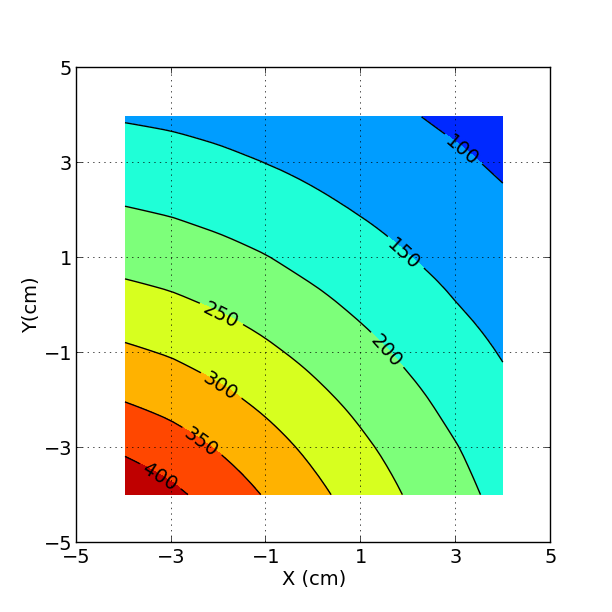
\includegraphics[width=\textwidth]{ZnO_profile.png}
\caption{\label{fig:1} ZnO calibration sample. Contours show film thickness (in nm).}
\end{minipage}
\hspace{0.5cm}
\begin{minipage}[b]{0.45\linewidth}
\centering
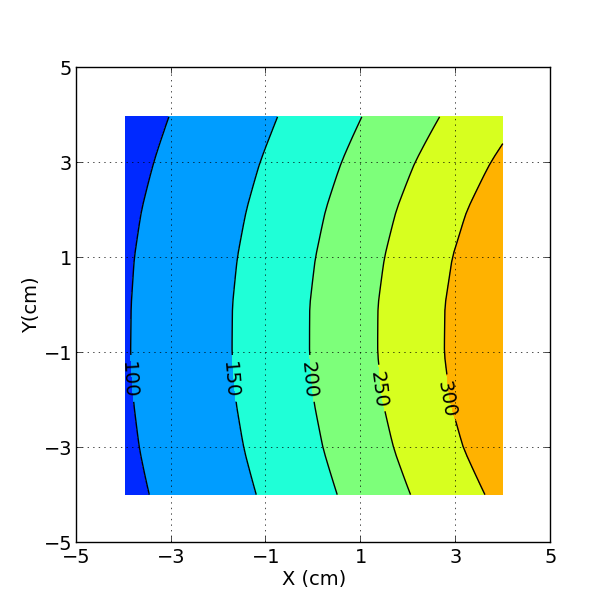
\includegraphics[width=\textwidth]{SnO2_profile.png}
\caption{\label{fig:2} SnO$_2$ calibration sample. Contours show film thickness (in nm).}
\end{minipage}
\end{figure}

\begin{figure}[ht]
\begin{minipage}[b]{0.45\linewidth}
\centering
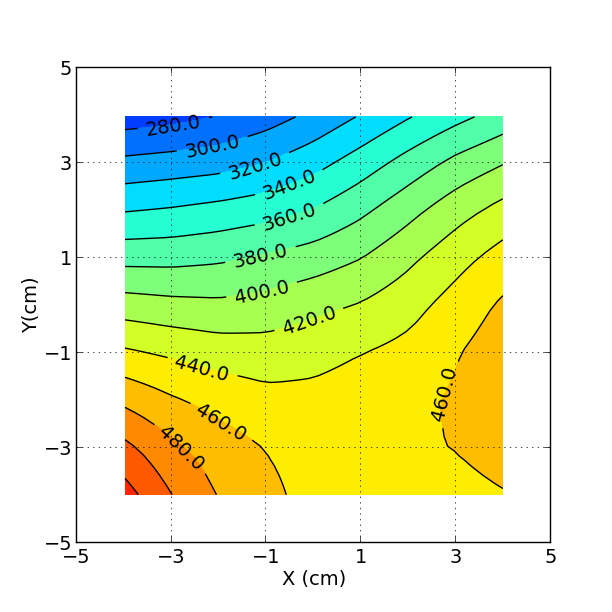
\includegraphics[width=\textwidth]{ZTO_profile_pred.png}
\caption{\label{fig:3} Calculated thickness of co-sputtered ZnO:SnO$_2$ film. Contours show film thickness (in nm).}
\end{minipage}
\hspace{0.5cm}
\begin{minipage}[b]{0.45\linewidth}
\centering
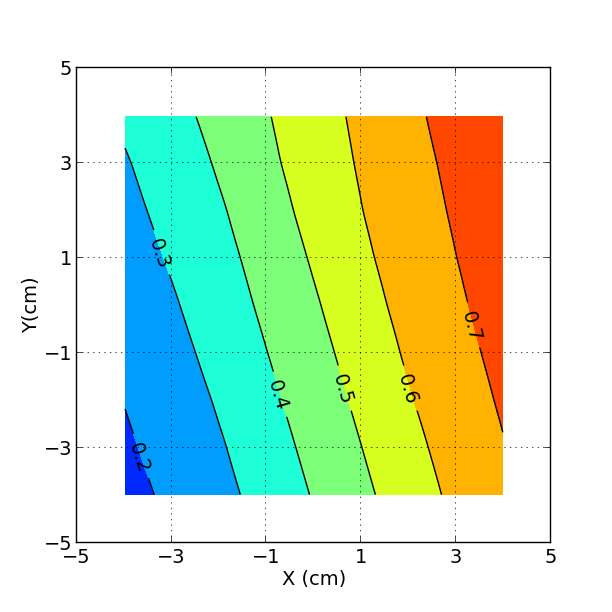
\includegraphics[width=\textwidth]{x_profile.png}
\caption{\label{fig:4} Profile of ratio $d_{SnO_{2}}/(d_{ZnO}+d_{SnO_{2}})$ calculated using figures \ref{fig:1} and \ref{fig:2}.}
\end{minipage}
\end{figure}


\begin{figure}[h]
    \centering
        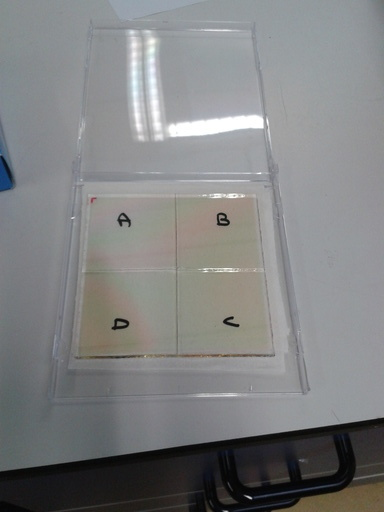
\includegraphics[width = 0.5\textwidth]{140220_2_rotate.jpg}
    \caption{Sample 140220\_2. Cut into 4 $5\times5$ cm$^2$ pieces. Orientation of sample in this photo corresponds directly with profile shown in figure \ref{fig:4}. Note: Film side is face-up in this photo.  }
\end{figure}

\begin{figure}[h]
    \centering
        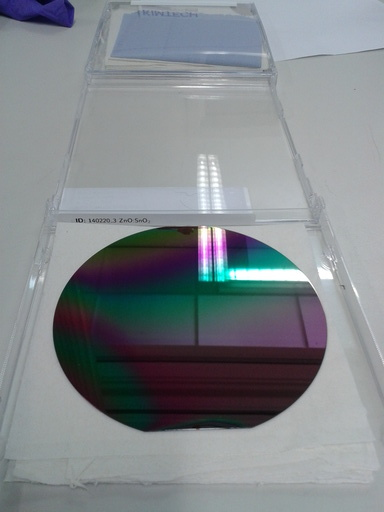
\includegraphics[width = 0.5\textwidth]{140220_3_rotate.jpg}
    \caption{Sample 140220\_3. Orientation of sample in this photo corresponds directly with the profile showin in figure \ref{fig:4}}
\end{figure}



\end{document}